\documentclass[../doc.tex]{subfiles}

\begin{document}

\section{Porównanie algorytmów wyszukiwania ścieżki}

\subsection{Symulacja}

Porównanie przeprowadzono na labiryncie o wymiarach \textbf{30×30}, wygenerowanym z wykorzystaniem \textbf{algorytmu Prima}. Punkty początkowy i końcowy zostały umieszczone odpowiednio na górnej i dolnej krawędzi planszy, co wymusza przejście przez całą jej wysokość. Strukturę wygenerowanego labiryntu przedstawiono na rysunku \ref{fig:test_maze}. 

Wyniki działania poszczególnych algorytmów wyszukiwania ścieżki zaprezentowano na rysunkach \ref{fig:dfs_maze}–\ref{fig:astar_maze} oraz w tabeli \ref{tab:simulation_result}.

\begin{figure}[H]
    \centering
    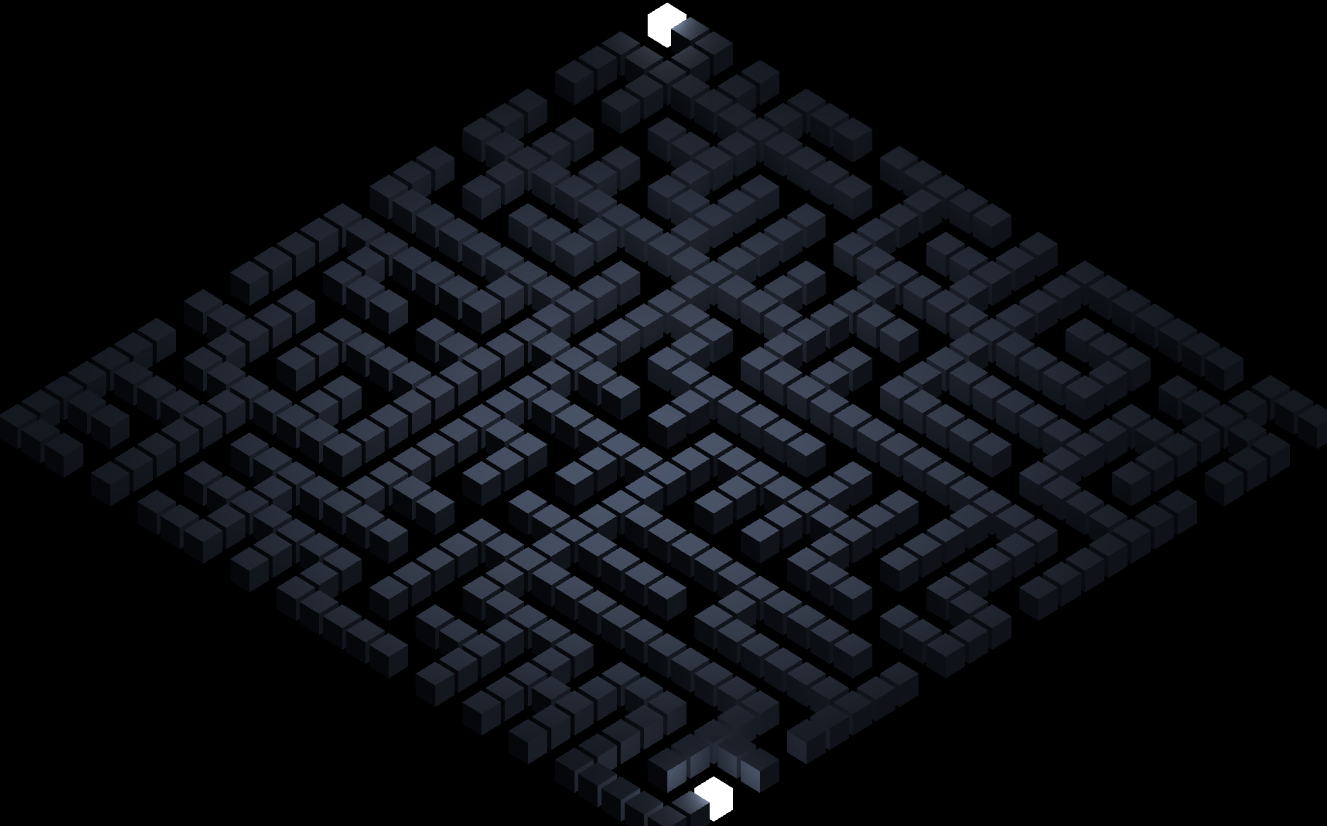
\includegraphics[width=0.85\textwidth]{figures/test_maze.png}
    \caption{Wygenerowany losowo labirynt, użyty w porównaniu.}
    \label{fig:test_maze}
\end{figure}

\begin{figure}[H]
    \centering
    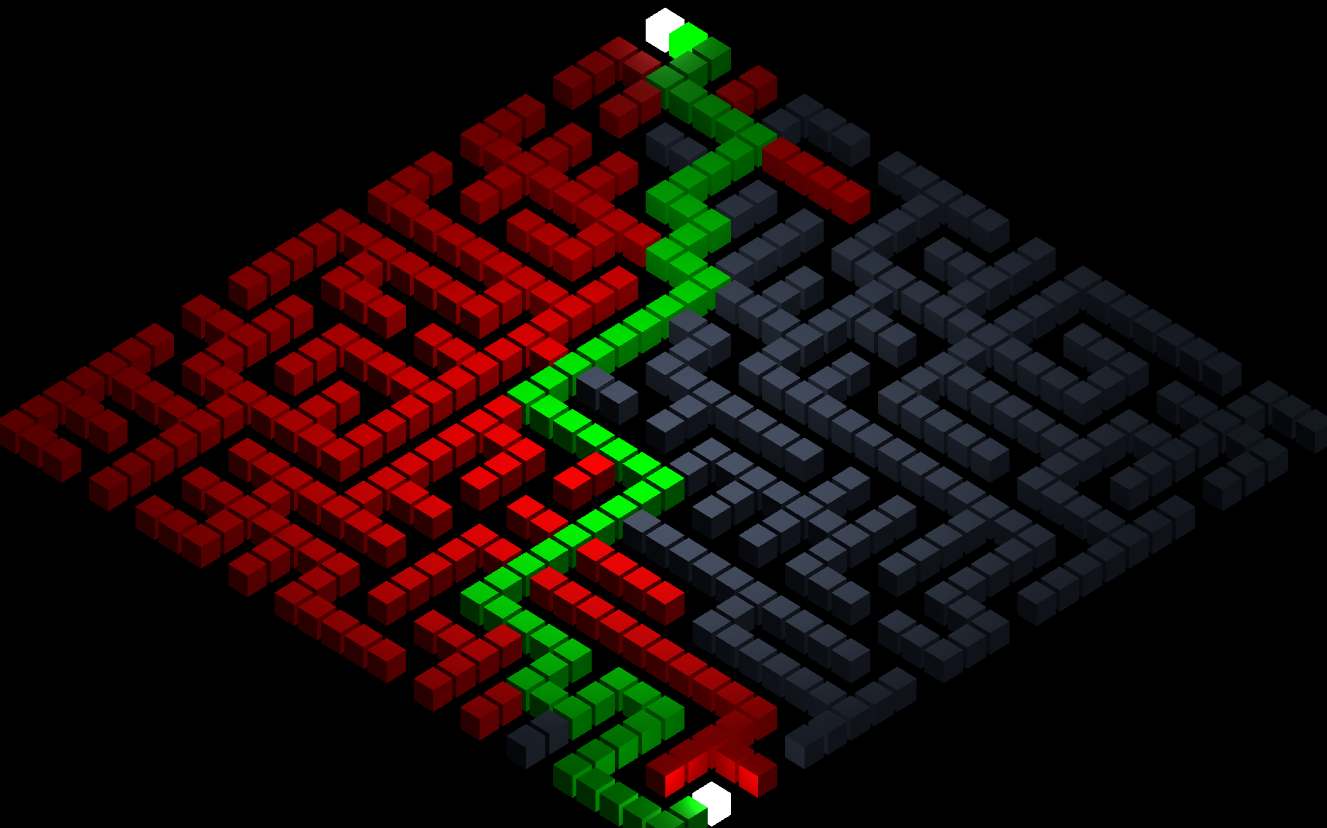
\includegraphics[width=0.85\textwidth]{figures/dfs.png}
    \caption{Wynik działania algorytmu DFS.}
    \label{fig:dfs_maze}
\end{figure}

\begin{figure}[H]
    \centering
    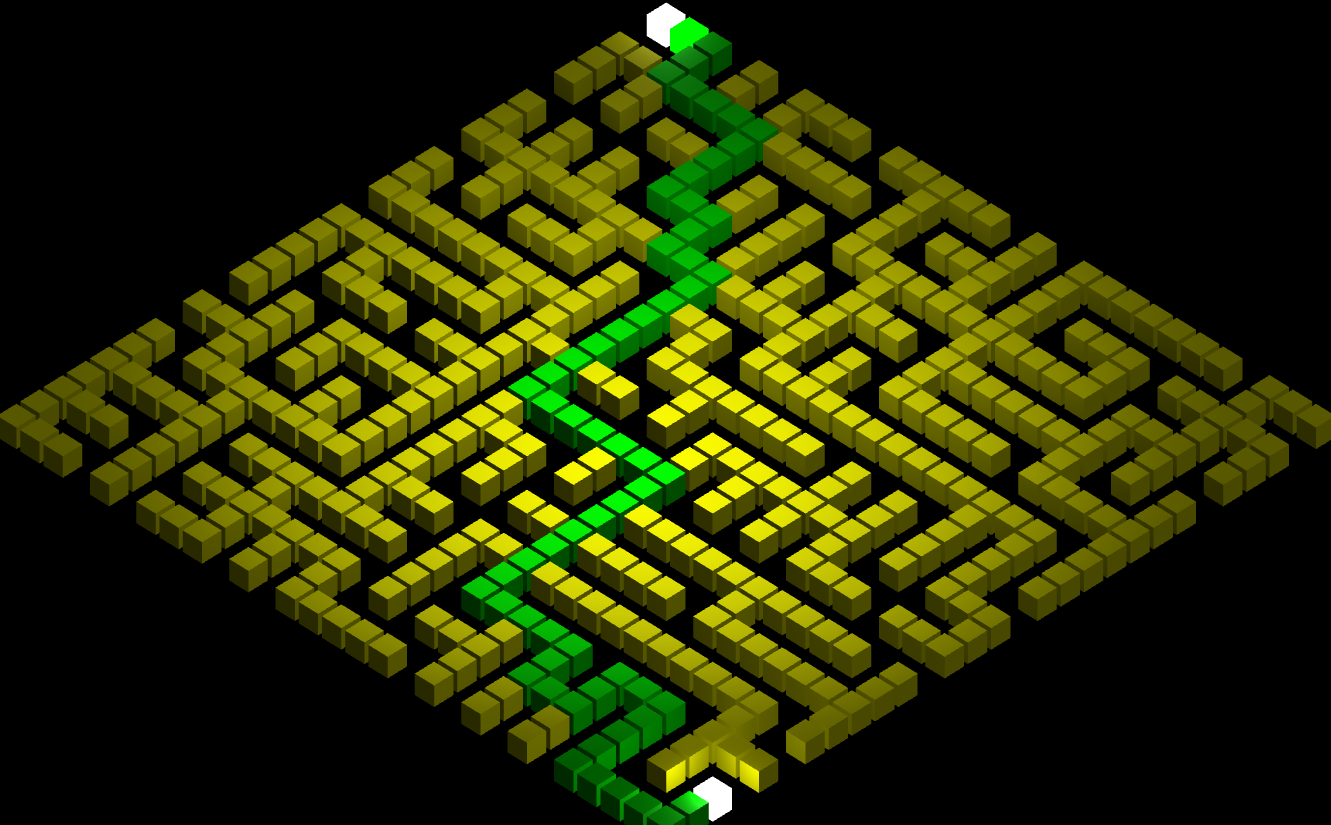
\includegraphics[width=0.85\textwidth]{figures/bfs.png}
    \caption{Wynik działania algorytmu BFS.}
    \label{fig:bfs_maze}
\end{figure}

\begin{figure}[H]
    \centering
    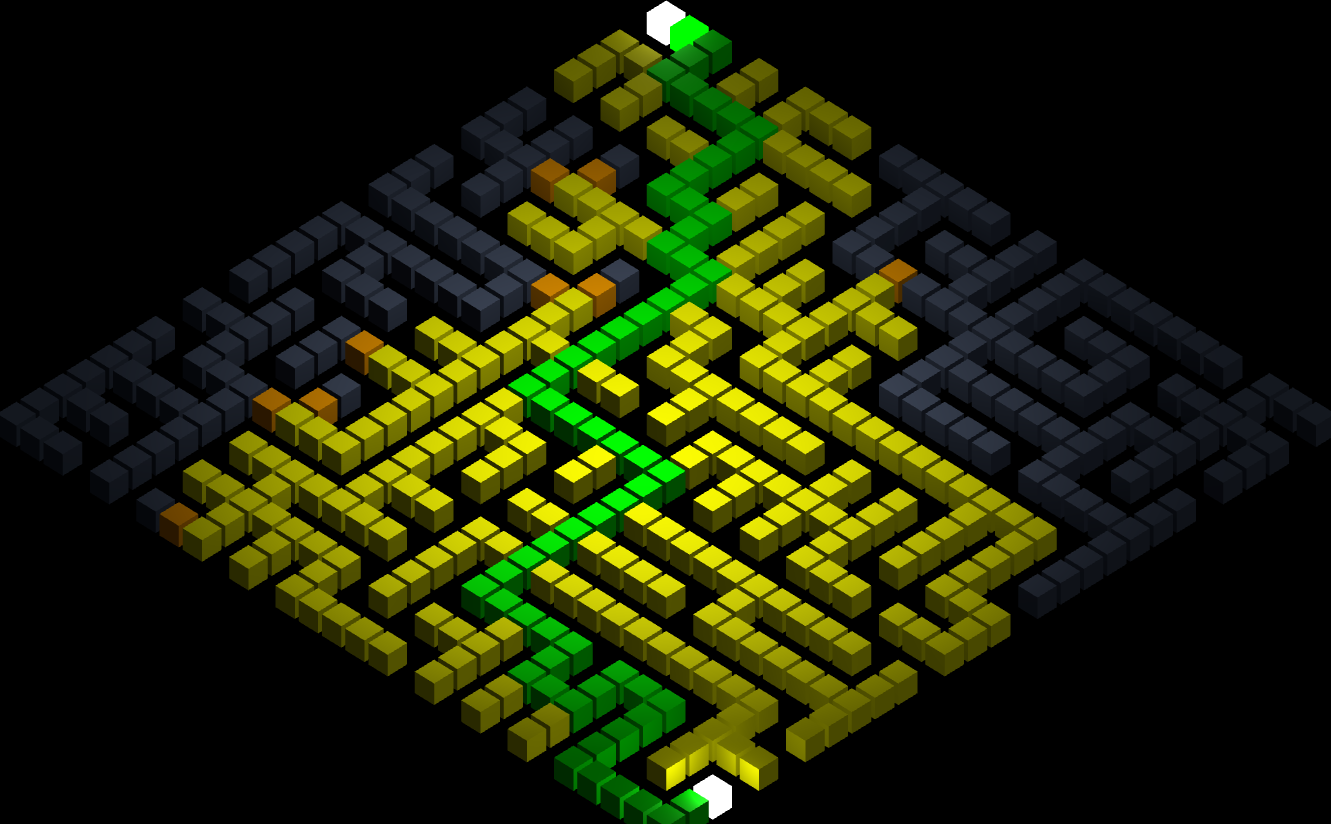
\includegraphics[width=0.85\textwidth]{figures/astar.png}
    \caption{Wynik działania algorytmu A*.}
    \label{fig:astar_maze}
\end{figure}

\begin{table}[H]
    \centering
    \begin{tabularx}{\textwidth}{|c|*{4}{>{\centering\arraybackslash}X|}c|}
        \hline
        \multirow{2}{*}{\textbf{Algorytm}} & \multicolumn{4}{c|}{\textbf{Ilość pól danej kategorii}} & \multirow{2}{*}{\parbox[c]{2cm}{\centering \textbf{Suma}\\ \textbf{kroków}}} \\ \cline{2-5}
                                           & \cellcolor{green!30} \textbf{\textit{Selected}} & \cellcolor{yellow!30} \textbf{\textit{Candidate}} & \cellcolor{orange!30} \textbf{\textit{Queued}} & \cellcolor{red!30}  \textbf{\textit{Forsaken}} &  \\ \hline
        DFS & 61 & 197 & 196 & 136 & 590 \\ \hline
        BFS & 61 & 447 & 446 & \multicolumn{1}{c|}{\textit{nie dotyczy}} & 954 \\ \hline
        A*  & 61 & 286 & 294 & \multicolumn{1}{c|}{\textit{nie dotyczy}} & 641 \\ \hline
    \end{tabularx}
    \caption{Wyniki działania poszczególnych algorytmów.}
    \label{tab:simulation_result}
\end{table}

\subsection{Interpretacja wyników}

Analiza danych zawartych w tabeli \ref{tab:simulation_result} pozwala na ocenę efektywności i charakterystyki działania poszczególnych algorytmów wyszukiwania ścieżki w kontekście złożoności przestrzeni przeszukiwania oraz liczby wykonanych operacji. Wszystkie trzy algorytmy – \textit{DFS}, \textit{BFS} oraz \textit{A*} – znalazły ścieżkę o identycznej długości (61 pól), co potwierdza poprawność ich implementacji oraz jednoznaczność najkrótszego rozwiązania w badanym labiryncie.

Z perspektywy liczby analizowanych pól (\textit{Candidate}) oraz pól dodanych do kolejki (\textit{Queued}), wyraźnie zauważalne są różnice w strategii działania poszczególnych metod. Algorytm BFS, przeszukujący przestrzeń wszerz, odznacza się największą liczbą aktywnie analizowanych pól (447) oraz bardzo dużym zasięgiem działania (446 pól w kolejce). Taka strategia zapewnia optymalność rozwiązania, ale wiąże się z wysokim kosztem obliczeniowym. 

DFS, jako algorytm oparty na przeszukiwaniu w głąb, wykazuje najniższą łączną liczbę kroków (590), jednak kosztem dużej liczby pól zakwalifikowanych jako \textit{Forsaken} (136). Wynika to z faktu, że DFS często „błądzi” w ślepe zaułki, które musi następnie porzucić, co skutkuje koniecznością cofania się i powtórnej eksploracji innych ścieżek. 

Algorytm A*, wykorzystujący heurystykę w ocenie kolejnych pól, stanowi kompromis pomiędzy szerokim przeszukiwaniem a kosztami obliczeniowymi. Choć przetwarza mniej pól niż BFS, to nadal zapewnia optymalną ścieżkę. Łączna liczba kroków (641) potwierdza jego wysoką efektywność w kontekście znalezienia najkrótszej trasy przy jednoczesnym ograniczeniu nadmiarowego przeszukiwania.

Podsumowując, algorytm A* okazał się najbardziej zrównoważony pod względem skuteczności oraz efektywności. BFS gwarantuje pełność i optymalność rozwiązania, jednak kosztem znacznie większej liczby operacji. DFS natomiast działa szybko i z mniejszym zużyciem zasobów, ale nie daje gwarancji optymalności i może znacząco wydłużyć czas przeszukiwania w bardziej złożonych przypadkach.


\end{document}